\documentclass[11pt]{article} %defining type of document you are creating %beamer is the type used for presentations %Here I'm defining font size (11 pt) as well.
%\usepackage{geometry}    %  adjust margins  
%\geometry{letterpaper}  %compile in the right dimensions          
\usepackage{graphicx} %package to include graphics
\usepackage{amssymb} %to type math
\usepackage{epstopdf} %to create pdf
\usepackage{url} %to include urls
\usepackage{hyperref} %to include hyperref
\usepackage{setspace} %to set line spacing


\title{Introduction to Latex}
\author{Nat\'alia Bueno}                               
%\date{}
% to exclude date, remove %

\begin{document}
\maketitle %creates a page for the title


\tableofcontents %created a table of contents 

\newpage %partes in a new page
% \noindent remove indentation
\noindent Today we are going to learn how to use a new typesetting program. The best way to learn is to create a template with commands. \LaTeX{} can be annoying at first, but then it becomes something that helps you to organize your own writing and your own \href{http://whatshouldwecallgradschool.tumblr.com/post/56277597781/why-i-do-research}{research}.
\\

We are going to cover the following things: 

\begin{itemize}
\item Creating bulleted lists
\item Changing fonts
\item Spacing, centering, and indentation
\item Typing equations
\item Including figures
\item Building a basic table
\end{itemize}

\vspace{4mm}
\section{Basic Formatting}

\vspace{4mm}
\subsection{Changing Fonts}

Sometimes when we write we want to put things in \emph{italics} or {\bf bold}.If you are old-fashioned, you can use \underline{underline}, but that is ugly. %\\ \\


%It doesn't matter how many empty lines you have, it will read as one. If you want more lines, use \\, as shown above 




Other times we would like to change the size                    of our fonts. Here is how you write {\tiny really small text.} Here is how you write {\huge really large text}.

%note how many empty spaces I havet here? It reads as one. 
%good ref for font sizes: http://www.sascha-frank.com/latex-font-size.html

\vspace{4mm}
\subsection{Spacing, Centering, and Indentation}

At any time, you can insert vertical space. 

\vspace{4mm}


I like to put space before my section headers. \hspace{10mm} I want horizontal space. 


\begin{center}
[Figure 1 About Here]
\end{center}

\doublespace

Now things are doublespaced. I put this at the beginning of my papers. 

\vspace{4mm}
\section{Advanced Environments}

Any time you type math, you can always just it in dollars signs. Our estimate of $\beta$ is $(X'X)^{-1}X'Y$.

\begin{equation}
\beta = (X'X)^{-1}X'Y
\end{equation}

\vspace{4mm}
\subsection{Figures}

You use figures with the figure environment. 

\begin{figure}[h!]
\caption{Everyone's favorite cartoon}
\vspace{6mm}
\centerline{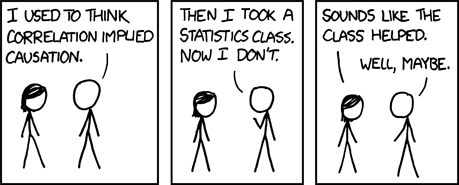
\includegraphics[scale=.5]{correlation.png}}
\end{figure}
\vspace{4mm}
\subsection{Tables}

Tables are the worst thing about \LaTeX{}  by far. 

\begin{table}[h]
\centering
\caption{My First Table}
\begin{tabular}{l c c c}
\\
\hline
\\
Low numbers & 1 & 2 & 3 \\
High numbers & 10 & 20 & 0 \\
\\
\hline
\end{tabular}
\end{table}

\section{Common mistakes}

\subsection*{Quotes}

Quotation marks in \LaTeX{}  files begin with two back ticks, ``, and end with two single quotes, ''. Not intuitive. 

{\bf Right}: ``Yes.''

{\bf Wrong}: "No."


\subsection*{Failure to use math mode} 

\LaTeX{} uses math mode to distinguish variables from ordinary letters. Variables are typeset in math italic, a special style that is not the same as ordinary italic prose.


{\bf Right}: Given a matrix $A$ and vector $b$, solve $Ax = b$.
and the second as

{\bf Wrong}: Given a matrix A and vector b, solve Ax = b.

\subsection*{Ellipses} 

This ... is wrong, but this \dots\ is better.

\subsection*{Foreign languages}

!`Adi\'os!
!`Cumplea\~nos!

\section{Acknowledgments and where to learn more:}

This practice is based on Rory Truex's materials as well as John Cook's blog posts.

\href{http://tobi.oetiker.ch/lshort/lshort.pdf}{The not so short introduction to \LaTeX{}}

\href{http://en.wikibooks.org/wiki/LaTeX/}{Wikibook} is your best friend.




\end{document}  